\documentclass[11pt]{article}
\usepackage[textwidth=18.0cm, textheight=23.0cm, top=2.0cm]{geometry}
\usepackage{pst-all}
\usepackage{amssymb}
\usepackage{tikz}
\usepackage{underscore}\begin{document}
\pagestyle{empty}


ClassName: \underline{\textbf{Class_05.2bp-3}}
\par
BinSize: \underline{\textbf{100 × 100}}
\par
ReduceSize: \underline{\textbf{100 × 100}}
\par
TypeNum: \underline{\textbf{20}}
\par
Num: \underline{\textbf{20}}
\par
OutS: \underline{\textbf{50000}}
\par
InS: \underline{\textbf{38889}}
\par
Rate: \underline{\textbf{0.778}}
\par
UB: \underline{\textbf{5}}
\par
LB0: \underline{\textbf{5}}
\par
LB: \underline{\textbf{5}}
\par
LBWithCut: \underline{\textbf{5}}
\par
NodeCut: \underline{\textbf{0}}
\par
ExtendedNodeCnt: \underline{\textbf{1}}
\par
GenNodeCnt: \underline{\textbf{1}}
\par
PrimalNode: \underline{\textbf{0}}
\par
ColumnCount: \underline{\textbf{5}}
\par
TotalCutCount: \underline{\textbf{0}}
\par
RootCutCount: \underline{\textbf{0}}
\par
LPSolverCnt: \underline{\textbf{1}}
\par
PricingSolverCnt: \underline{\textbf{0}}
\par
BranchAndBoundNum: \underline{\textbf{1}}
\par
isOpt: \underline{\textbf{true}}
\par
TimeOnInitSolution: \underline{\textbf{600.000 s}}
\par
TimeOnPrimal: \underline{\textbf{0.000 s}}
\par
TimeOnPricing: \underline{\textbf{0.000 s}}
\par
TimeOnRmp: \underline{\textbf{0.062 s}}
\par
TotalTime: \underline{\textbf{600.359 s}}
\par
\newpage


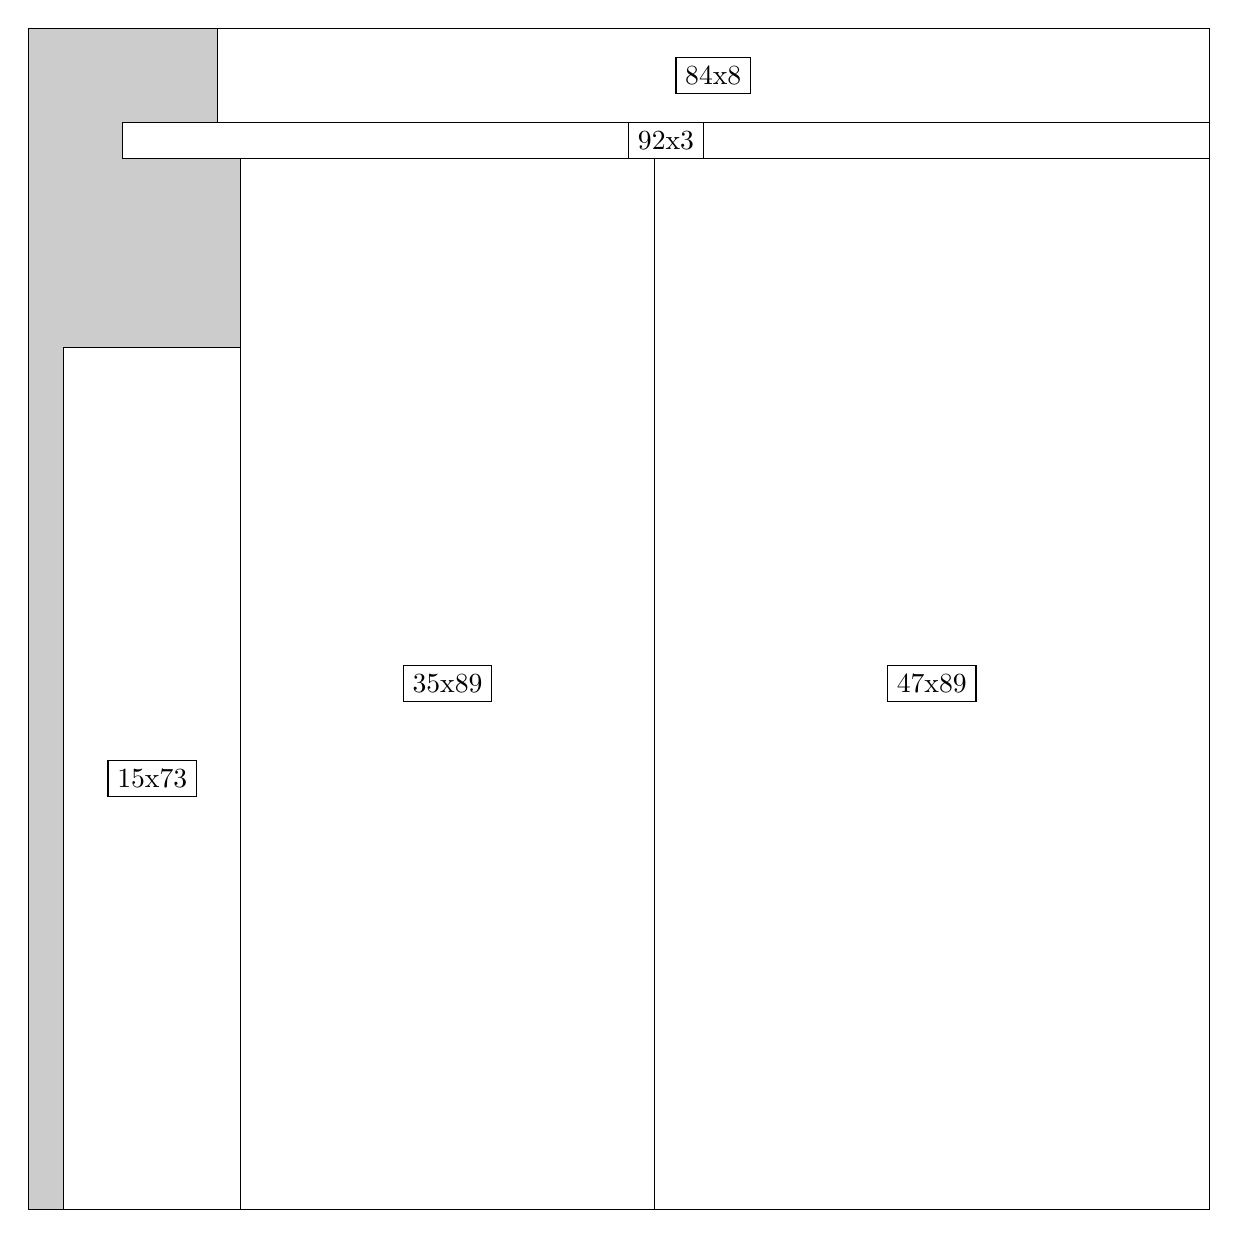
\begin{tikzpicture}[shorten >=1pt,scale=1.0,every node/.style={scale=1.0},->]
\tikzstyle{vertex}=[circle,fill=black!25,minimum size=14pt,inner sep=0pt]
\filldraw[fill=gray!40!white, draw=black] (0,0) rectangle (15.0,15.0);
\foreach \name/\x/\y/\w/\h in {47x89/7.949999999999999/0.0/7.05/13.35,35x89/2.6999999999999997/0.0/5.25/13.35,15x73/0.44999999999999996/0.0/2.25/10.95,92x3/1.2/13.35/13.799999999999999/0.44999999999999996,84x8/2.4/13.799999999999999/12.6/1.2}
\filldraw[fill=white!40!white, draw=black] (\x,\y) rectangle node[draw] (\name) {\name} ++(\w,\h);
\end{tikzpicture}


w =47 , h =89 , x =53 , y =0 , v =4183
\par
w =35 , h =89 , x =18 , y =0 , v =3115
\par
w =15 , h =73 , x =3 , y =0 , v =1095
\par
w =92 , h =3 , x =8 , y =89 , v =276
\par
w =84 , h =8 , x =16 , y =92 , v =672
\par
\newpage


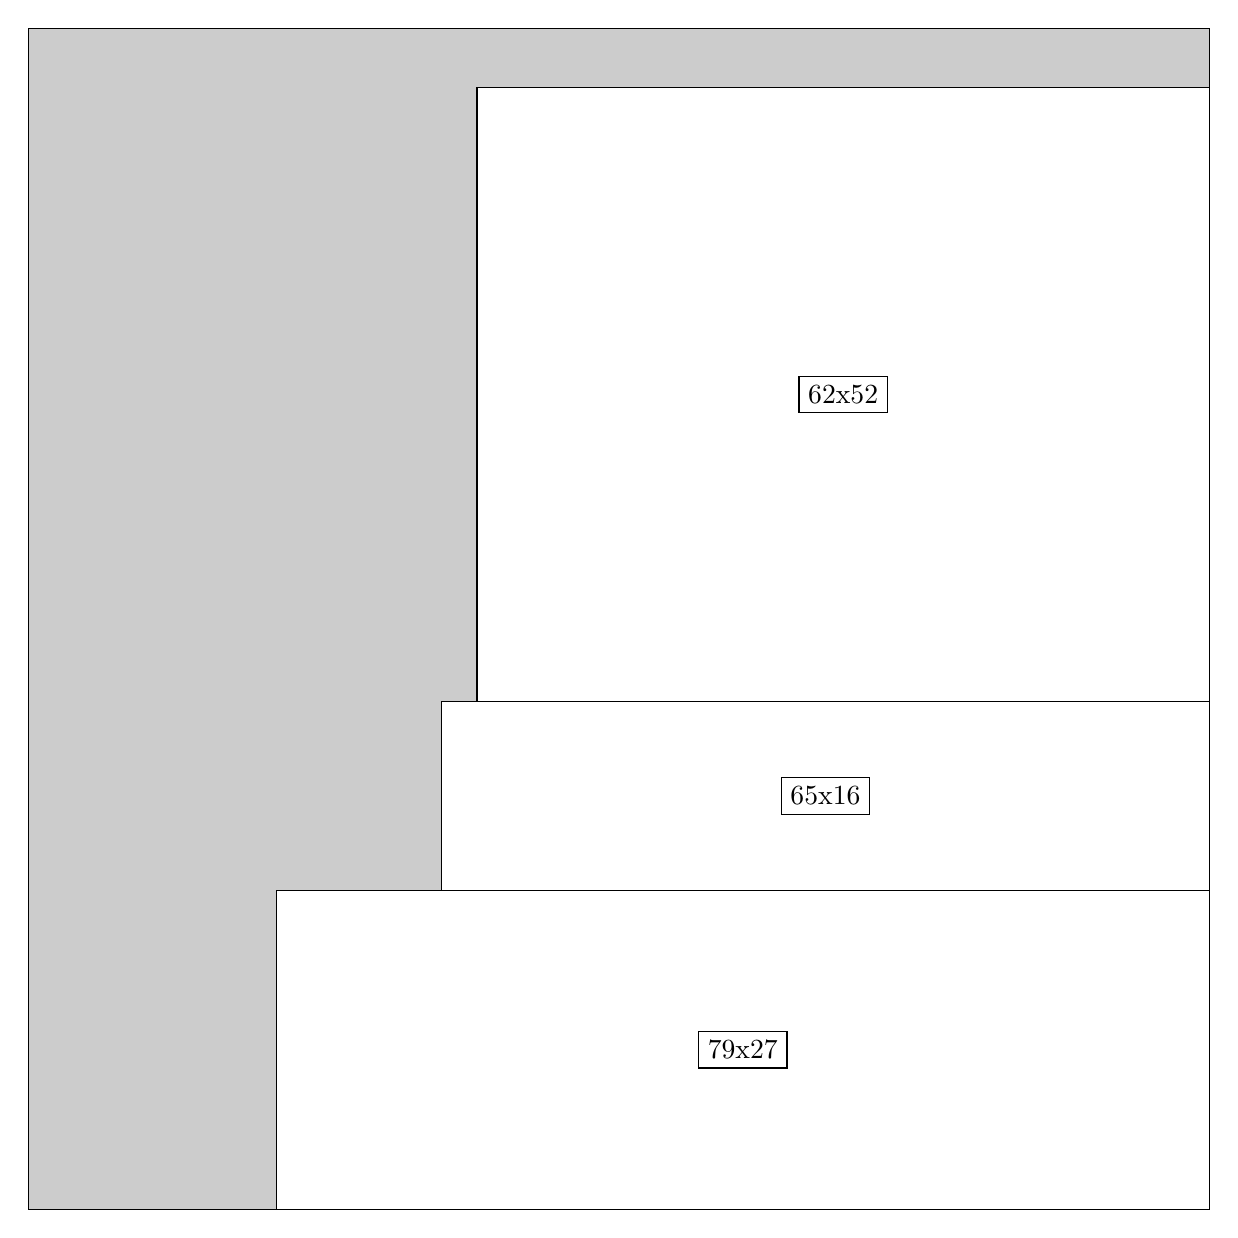
\begin{tikzpicture}[shorten >=1pt,scale=1.0,every node/.style={scale=1.0},->]
\tikzstyle{vertex}=[circle,fill=black!25,minimum size=14pt,inner sep=0pt]
\filldraw[fill=gray!40!white, draw=black] (0,0) rectangle (15.0,15.0);
\foreach \name/\x/\y/\w/\h in {79x27/3.15/0.0/11.85/4.05,65x16/5.25/4.05/9.75/2.4,62x52/5.7/6.45/9.299999999999999/7.8}
\filldraw[fill=white!40!white, draw=black] (\x,\y) rectangle node[draw] (\name) {\name} ++(\w,\h);
\end{tikzpicture}


w =79 , h =27 , x =21 , y =0 , v =2133
\par
w =65 , h =16 , x =35 , y =27 , v =1040
\par
w =62 , h =52 , x =38 , y =43 , v =3224
\par
\newpage


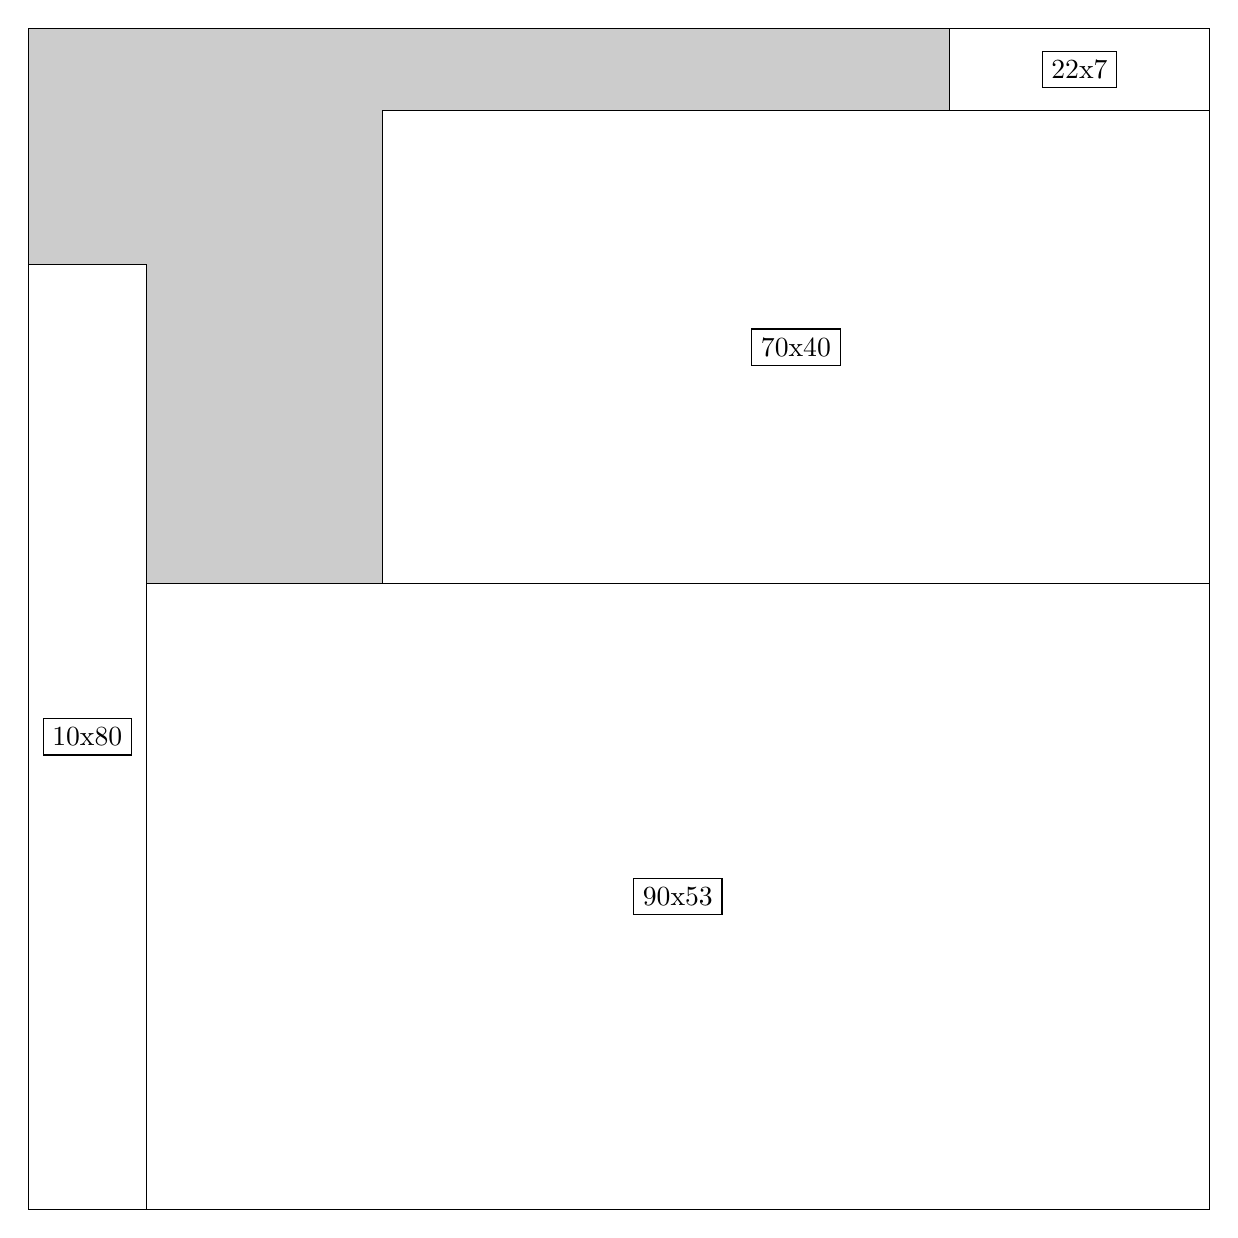
\begin{tikzpicture}[shorten >=1pt,scale=1.0,every node/.style={scale=1.0},->]
\tikzstyle{vertex}=[circle,fill=black!25,minimum size=14pt,inner sep=0pt]
\filldraw[fill=gray!40!white, draw=black] (0,0) rectangle (15.0,15.0);
\foreach \name/\x/\y/\w/\h in {90x53/1.5/0.0/13.5/7.949999999999999,70x40/4.5/7.949999999999999/10.5/6.0,22x7/11.7/13.95/3.3/1.05,10x80/0.0/0.0/1.5/12.0}
\filldraw[fill=white!40!white, draw=black] (\x,\y) rectangle node[draw] (\name) {\name} ++(\w,\h);
\end{tikzpicture}


w =90 , h =53 , x =10 , y =0 , v =4770
\par
w =70 , h =40 , x =30 , y =53 , v =2800
\par
w =22 , h =7 , x =78 , y =93 , v =154
\par
w =10 , h =80 , x =0 , y =0 , v =800
\par
\newpage


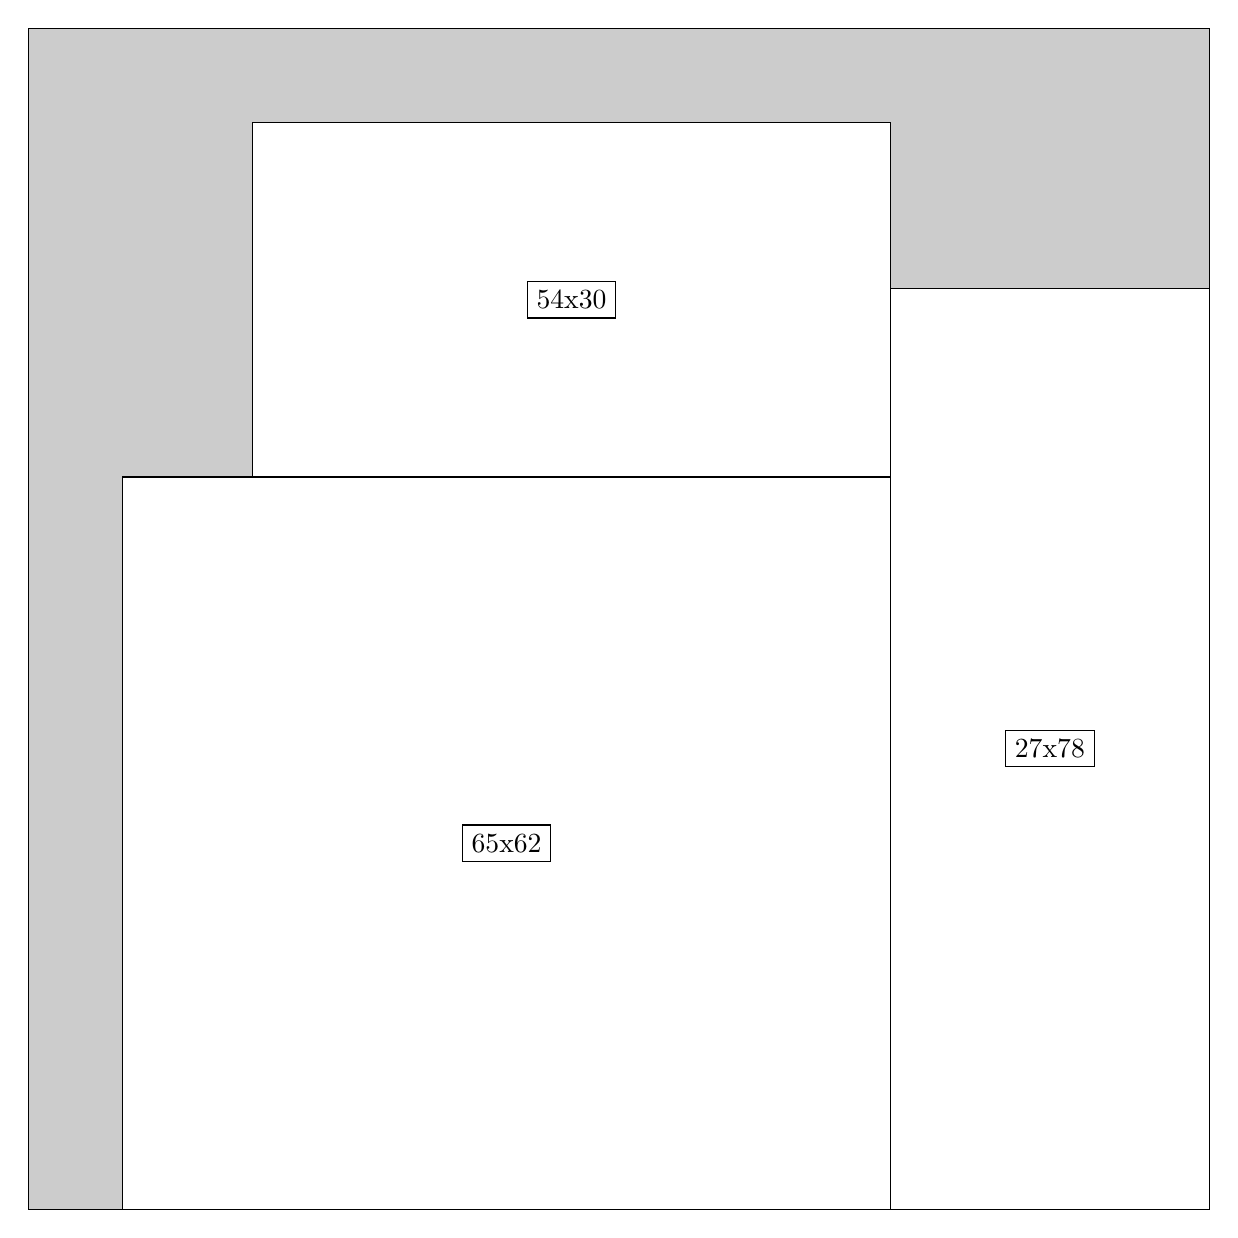
\begin{tikzpicture}[shorten >=1pt,scale=1.0,every node/.style={scale=1.0},->]
\tikzstyle{vertex}=[circle,fill=black!25,minimum size=14pt,inner sep=0pt]
\filldraw[fill=gray!40!white, draw=black] (0,0) rectangle (15.0,15.0);
\foreach \name/\x/\y/\w/\h in {27x78/10.95/0.0/4.05/11.7,65x62/1.2/0.0/9.75/9.299999999999999,54x30/2.85/9.299999999999999/8.1/4.5}
\filldraw[fill=white!40!white, draw=black] (\x,\y) rectangle node[draw] (\name) {\name} ++(\w,\h);
\end{tikzpicture}


w =27 , h =78 , x =73 , y =0 , v =2106
\par
w =65 , h =62 , x =8 , y =0 , v =4030
\par
w =54 , h =30 , x =19 , y =62 , v =1620
\par
\newpage


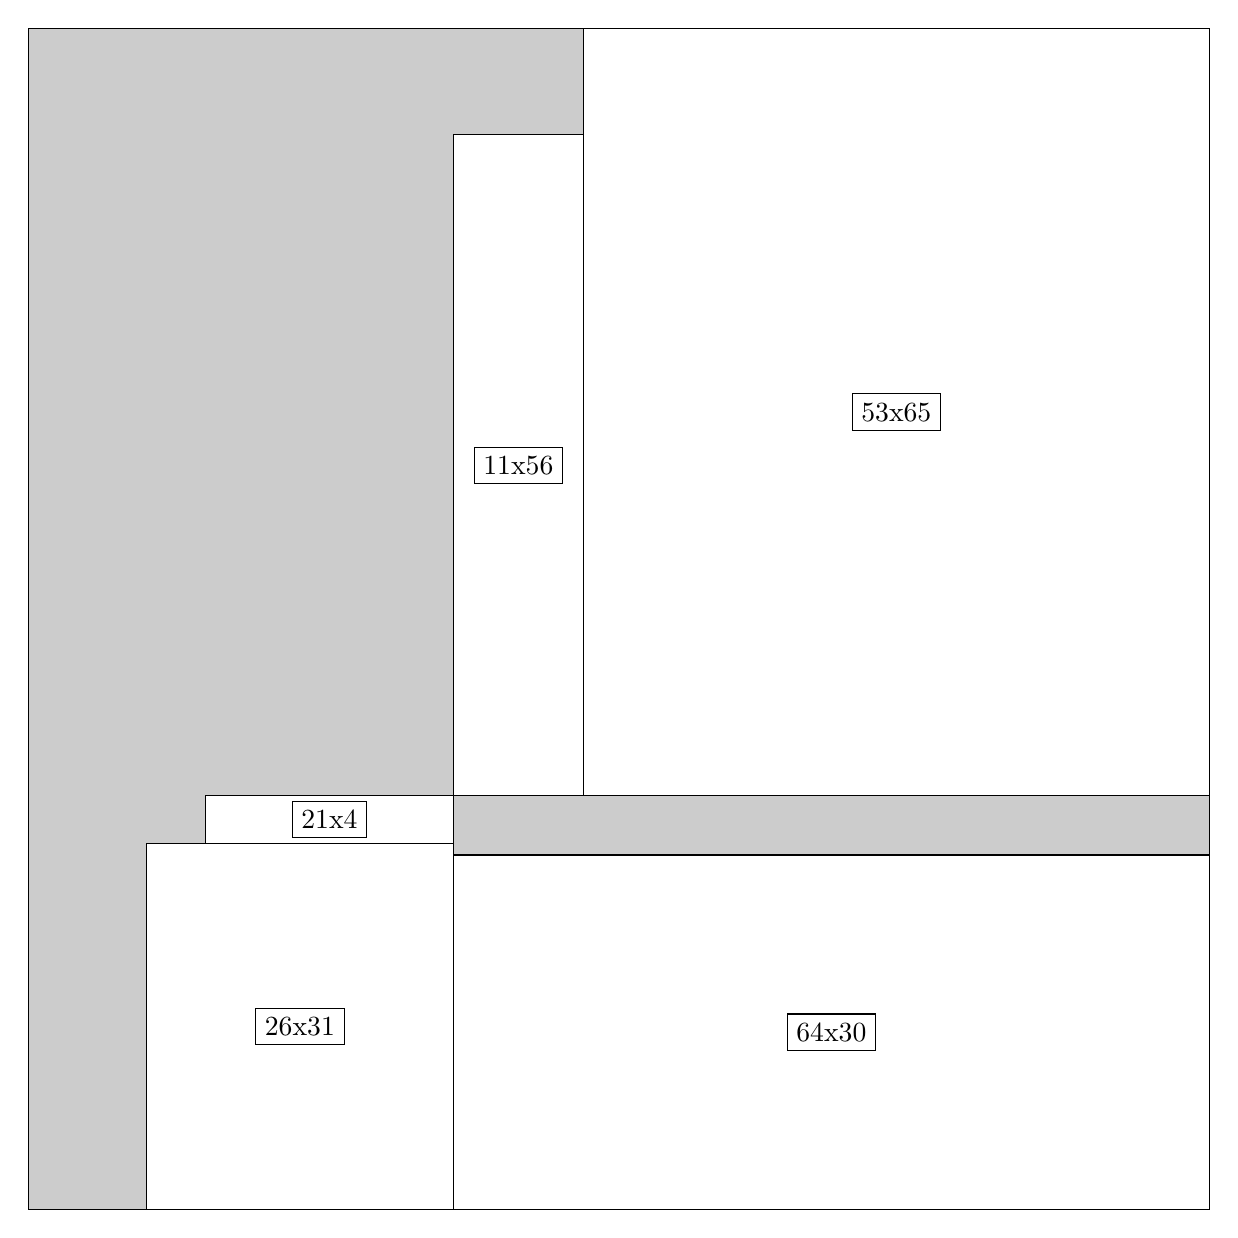
\begin{tikzpicture}[shorten >=1pt,scale=1.0,every node/.style={scale=1.0},->]
\tikzstyle{vertex}=[circle,fill=black!25,minimum size=14pt,inner sep=0pt]
\filldraw[fill=gray!40!white, draw=black] (0,0) rectangle (15.0,15.0);
\foreach \name/\x/\y/\w/\h in {64x30/5.3999999999999995/0.0/9.6/4.5,26x31/1.5/0.0/3.9/4.6499999999999995,21x4/2.25/4.6499999999999995/3.15/0.6,53x65/7.05/5.25/7.949999999999999/9.75,11x56/5.3999999999999995/5.25/1.65/8.4}
\filldraw[fill=white!40!white, draw=black] (\x,\y) rectangle node[draw] (\name) {\name} ++(\w,\h);
\end{tikzpicture}


w =64 , h =30 , x =36 , y =0 , v =1920
\par
w =26 , h =31 , x =10 , y =0 , v =806
\par
w =21 , h =4 , x =15 , y =31 , v =84
\par
w =53 , h =65 , x =47 , y =35 , v =3445
\par
w =11 , h =56 , x =36 , y =35 , v =616
\par
\newpage


\end{document}